\documentclass[serif,mathserif, french]{beamer}
\usepackage{amsmath, amsfonts, epsfig, xspace}
\usepackage[utf8]{inputenc}
\usepackage[french]{babel}
\usepackage{algorithm,algorithmic}
\usepackage{pstricks,pst-node}
\usepackage{multimedia}
\usepackage{listings}
\usepackage[normal,tight,center]{subfigure}
\setlength{\subfigcapskip}{-.5em}
\usepackage{beamerthemesplit}
\usetheme{lankton-keynote}

\author[Samuel Riedo \& Pascal Roulin]{Samuel Riedo \quad Pascal Roulin}

\title[Space Invaders\hspace{2em}\insertframenumber/\inserttotalframenumber]{Space Invaders}

\date{\today}

\institute{Justice League of VHDL}

\begin{document}

\maketitle

% \section{Introduction}  % add these to see outline in slides

\begin{frame}
  \frametitle{Sommaire}
  \begin{itemize}
  \item Introduction
  \item Le jeu
  \item Architecture
  \item Simulation
  \item Problèmes rencontrés
  \item Question
  \item Démonstration
  \end{itemize}
\end{frame}

\begin{frame}
  \frametitle{Introduction}
  \begin{itemize}
  \item Créer un projet complet en VHDL
  \item Utiliser la technologie VGA
  \item Valider le fonctionnement avec des testbenchs
  \end{itemize}
\end{frame}

\begin{frame}
  \frametitle{Le jeu}
  \begin{itemize}
  \item Jeu vidéo d'arcade
  \item Shoot 'em up
  \item 1978
  \item 2D
  \item Nombreuses versions
  \end{itemize}
  \begin{center}
  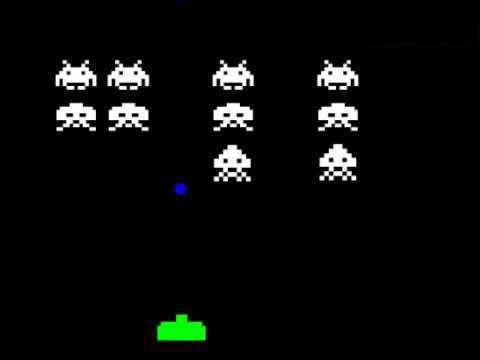
\includegraphics[width=.5\linewidth]{gameOnArcade}
  \end{center}
\end{frame}

\begin{frame}
  \frametitle{Architecture}
  \begin{center}
      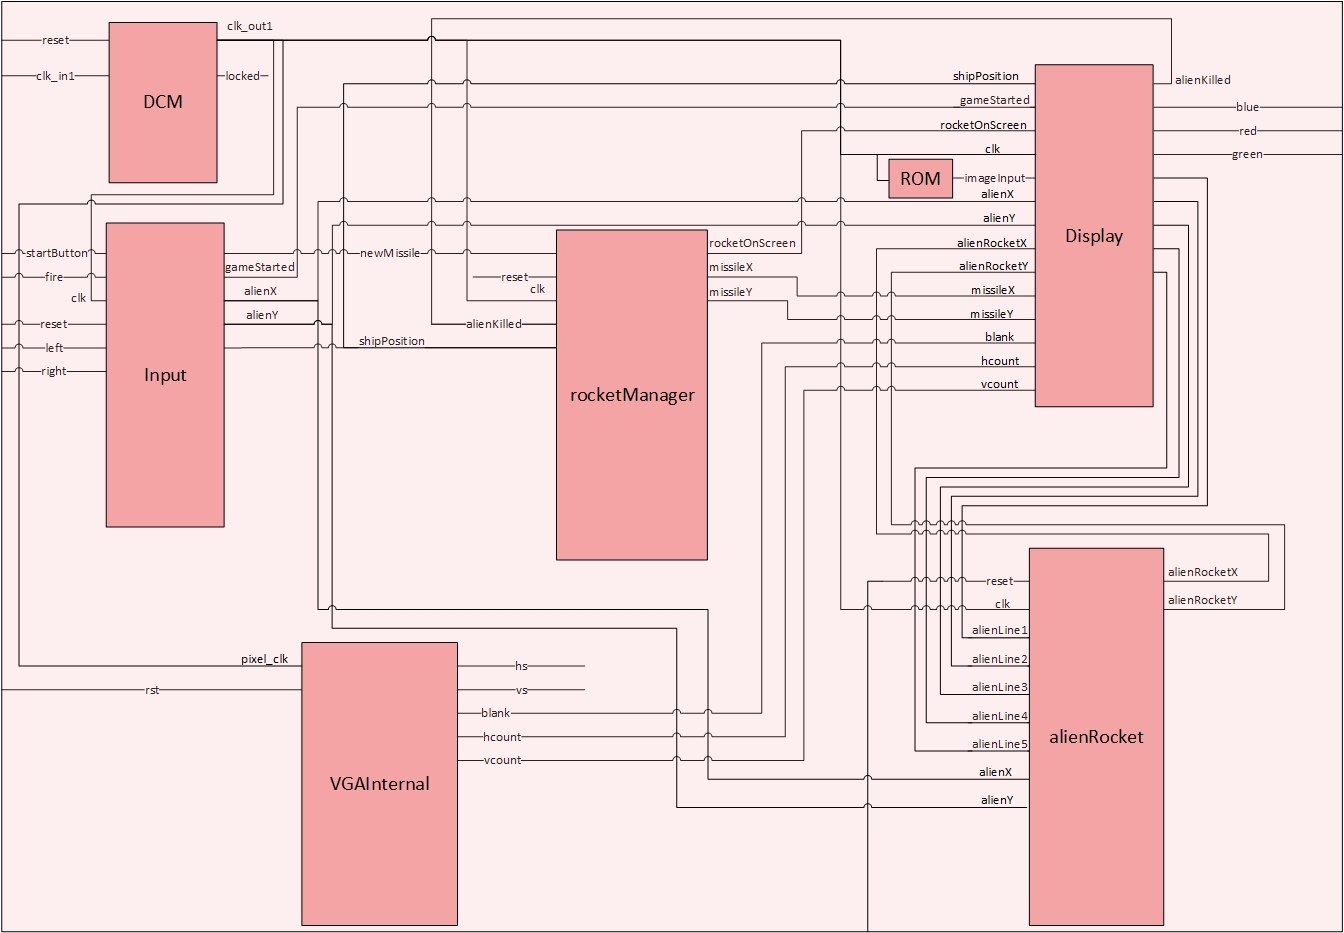
\includegraphics[width=\linewidth]{TopModuleArchitecture}
      \end{center}
\end{frame}

\begin{frame}
  \frametitle{Gestion des aliens}
  \begin{center}
      
\includegraphics[width=\linewidth]{aliens}
      \end{center}
\end{frame}

\begin{frame}
  \frametitle{Simulation}
  \begin{itemize}
  \item Tests pratiques
  \item Méthode Agile
  \item Testbenchs sur la version finale
  \end{itemize}
\end{frame}

\begin{frame}[fragile]
  \frametitle{Problèmes rencontrés}
  \begin{itemize}
  \item Hardware limité (RAM \& ROM)
  \item Modulo
  \item Accès dynamique aux données
  \item Accès à la clock 100MHz en dehors du DCM
  \item Génération d'aléatoire sans séquences
  \end{itemize}
  
  \begin{lstlisting}[frame=single, basicstyle=\tiny]
  -- This compile
  alienIndex <= (((hcounter-alienXX)/30) mod 10) when (hcounter-alienXX) >= 0 else 0;
  
  -- This doesn't
  alienLine <= (((vcounter-alienYY)/30) mod 5) when (vcounter-alienYY) >= 0 else 0;
  
  -- This trick does the same thing, but compile
  temp      <= (vcounter-alienYY) when (vcounter-alienYY) >= 0 else 0;
  temp2     <= temp / 30;
  temp3     <= temp2 mod 5;
  alienLine <= temp3;
  \end{lstlisting}
\end{frame}

\begin{frame}
  \frametitle{Conclusion}
  \begin{itemize}
  \item Projet intéressant et motivant
  \item Mise en pratique de la matière du cours
  \item Autogestion du planning 
  \end{itemize}
\end{frame}

\begin{frame}
  \frametitle{Questions}
      \begin{center}
      
\includegraphics[width=.4\linewidth]{question}
      \end{center}
\end{frame}

\begin{frame}
  \frametitle{Démonstration}
    \begin{center}
      
\includegraphics[width=.7\linewidth]{startScreen}
      \end{center}
\end{frame}


\end{document}
